\section{Anwendungen}
\subsection{Totale und Bedingte Wahrscheinlichkeit - HIV}
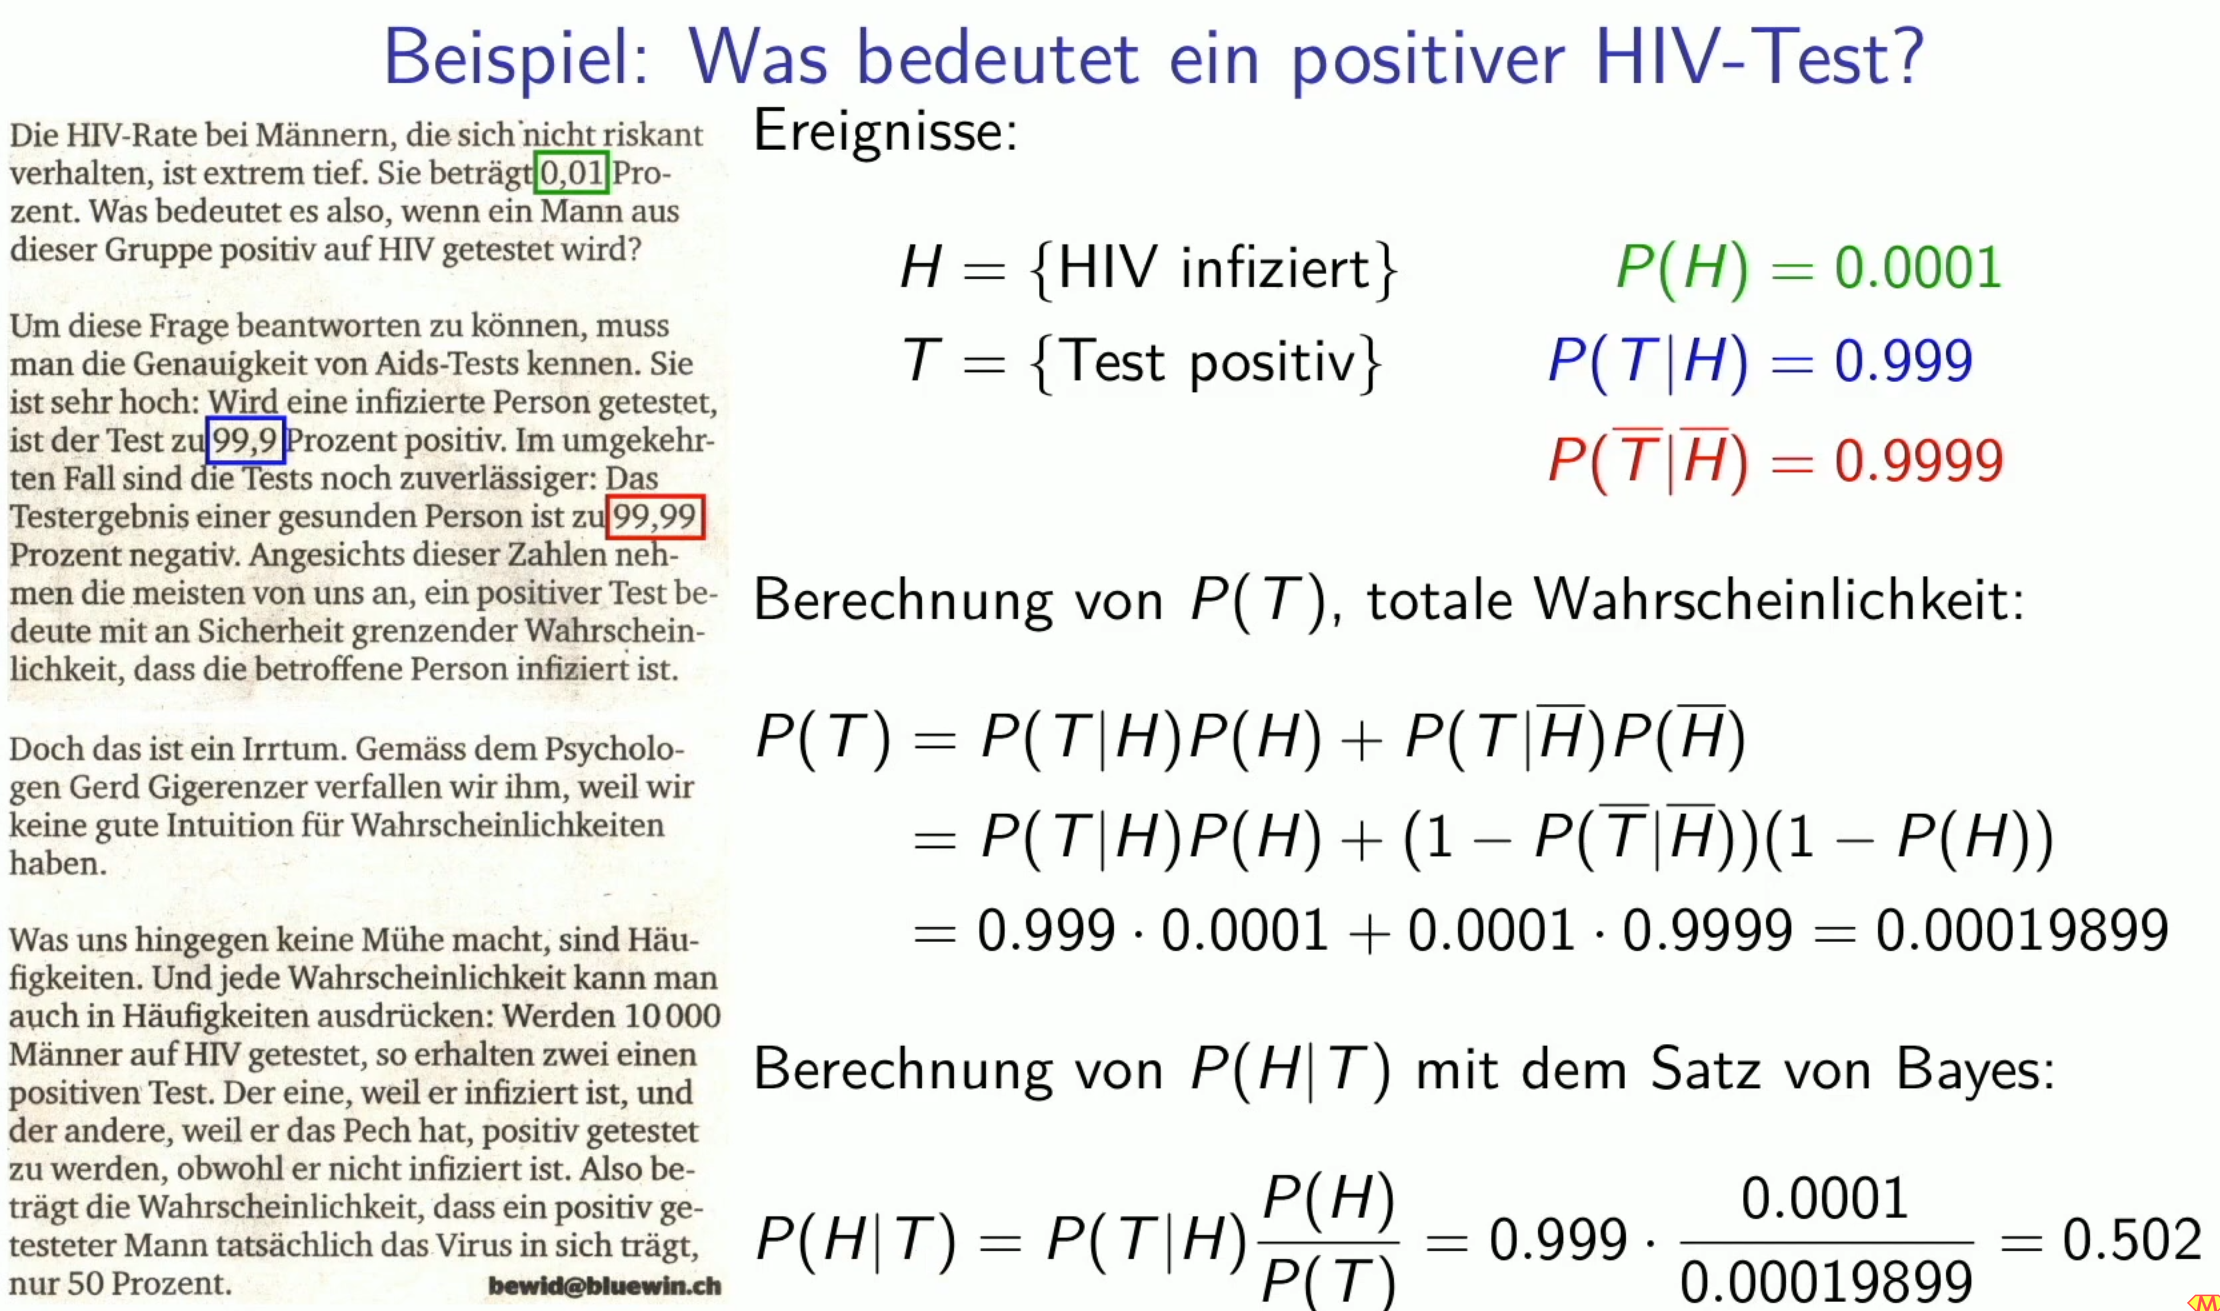
\includegraphics[width=\linewidth]{Images/HIV}

\subsection{Wahrscheinlichkeitsdichte}
\todo{Woche 6: Prüfungsaufgabe: Wahrscheinlichkeitsdichte muss 1 sein, Paramter anpassen.}

\subsection{Binomialverteilung Approximation}
\subsubsection{Normalverteilung}\label{approx_normal}
\todo{Beispiel Prüfung 2020 Aufgabe 6.} 

\subsubsection{Poissionverteilung}\label{approx_poission}
\todo{Beispiel Prüfung 2020 Aufgabe 6.} 

\subsection{Schätzen}\label{konf_intervall}
\todo{Beispiel Prüfung 2020\\
	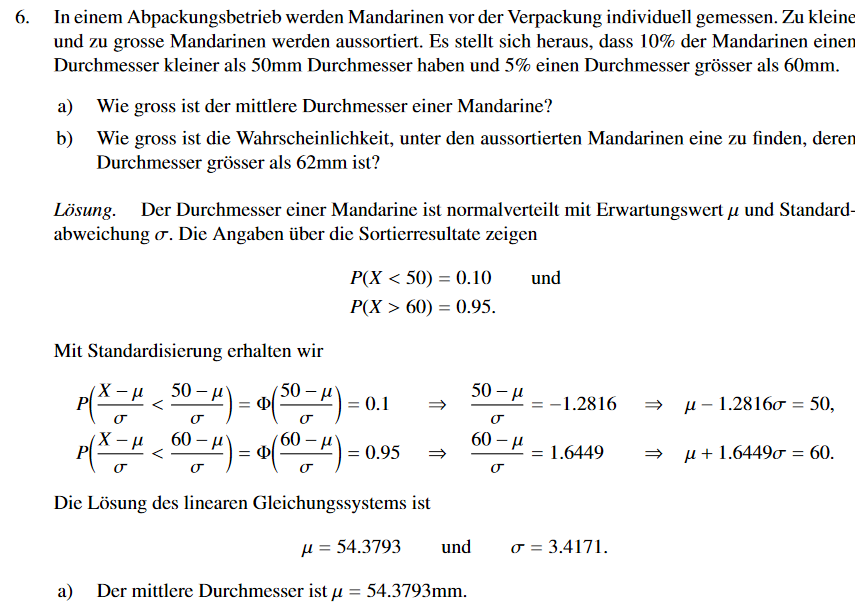
\includegraphics[width=\columnwidth]{Images/screenshot001}
}


\subsection{Linear Regression}\label{covarianz_eg}\label{regression}
Eine Regression bewerten. Die Geradenkoeffizienten $ a= 0.6278, b = 7.385$ wurden mit LeastSquare gefunden.
\begin{center}
	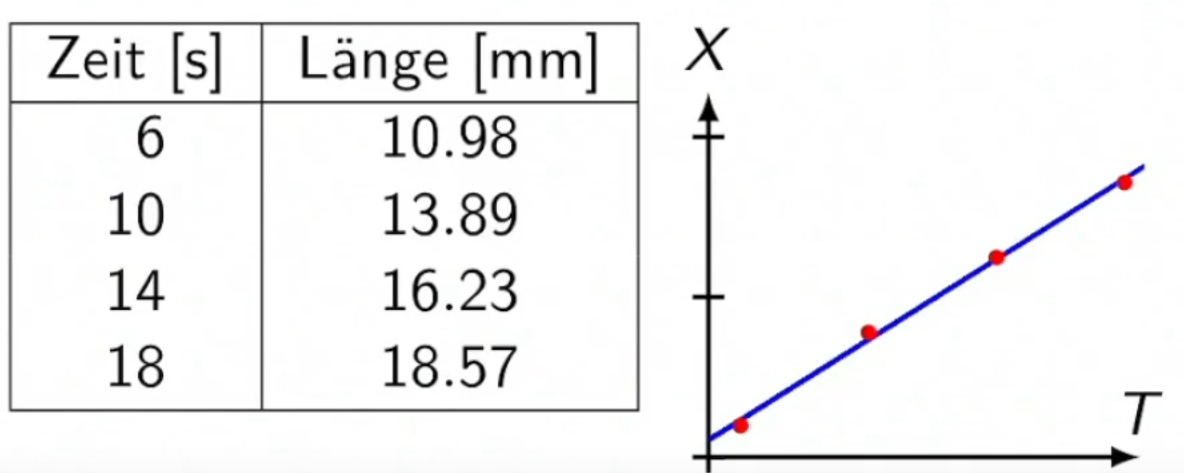
\includegraphics[width=0.5\columnwidth]{Images/regression}
\end{center}

\begin{center}
	\begin{tabular}{l|rr|rr|r}
		$j$ & $t_j$ & $t^2_j$ & $x_i$ & $x_i^2$ & $t_jx_j$ \\ \toprule
		1 & 6 & 36 & 10.98 & 120.6 & 65.88 \\  \midrule
		2 & 10 & 100 & 13.89 & 192.9 & 138.9 \\  \midrule
		3 & 14 & 196 & 16.23 & 263.4 & 227.2\\  \midrule
		4 & 18 & 324 & 18.57 & 344.8 & 334.3 \\  \bottomrule
		$\sum$  & 48 & 656 &  59.67 & 921.74 & 766.26\
	\end{tabular}
\end{center}

\noindent Daraus lassen sich folgende Werte bestimmen:
\begin{align*}
	E(t) &= 12 \qquad E(t^2) = 164  \\
	E(x) &= 14.91 \qquad E(x)^2 = 230.44  \\
	\cov(T, X) &= E(tx) - E(x)E(t) = 191.56 - (14.91 \cdot 12) = 12.56 \\
	\var(t) &= E(t^2) - E(t)^2 = 164 - 144 = 20 \\
	\var(x) &= E(x^2) - E(x)^2 = 230.4 - 222.3 = 8.129 \\
	r^2 &= \frac{\cov(t, x)^2}{\var(t)\var(x)} = \frac{12.56^2}{20\cdot 8.129} = 0.9695
\end{align*}

\noindent Der Wert liegt nahe bei $1$, daher eine recht gute Regression.

\subsection{Hypergeometrische Verteilung}
In einer Kiste mit 20 Äpfeln sind 5 wurmstichig. Wie gross ist die Wahrscheinlichkeit, in einer Stichprobe von 8 Äpfeln 2 wurmstichige zu funden? $N= 20, M = 5, n = 8, m = 2$
\[
P(X= 2) = \frac{\begin{pmatrix} 5 \\ 2 \end{pmatrix}\begin{pmatrix} 15 \\ 6 \end{pmatrix}}{\begin{pmatrix} 20 \\ 8 \end{pmatrix}} = 0.3973
\]


\subsection{Testen einer Verteilung}
\subsubsection{$\chi^2$-Test}\label{tictac}
\textbf{Nullhypothese} $H_0$: Alle Farben sind im TicTac gleich wahrscheinlich, d.h. $p_i = \frac{1}{4}$.\\
Die \textbf{Parameter} sind $4$ Farben, daraus ergeben sich $k= 4 -1 = 3$ Freiheitsgrade. $\alpha = 0.05$ wird in diesem Fall angenommen. Aus der $\chi^2$Tabelle ergibt den Kritischen $D_\text{krit} = 7.815$
\begin{center}
	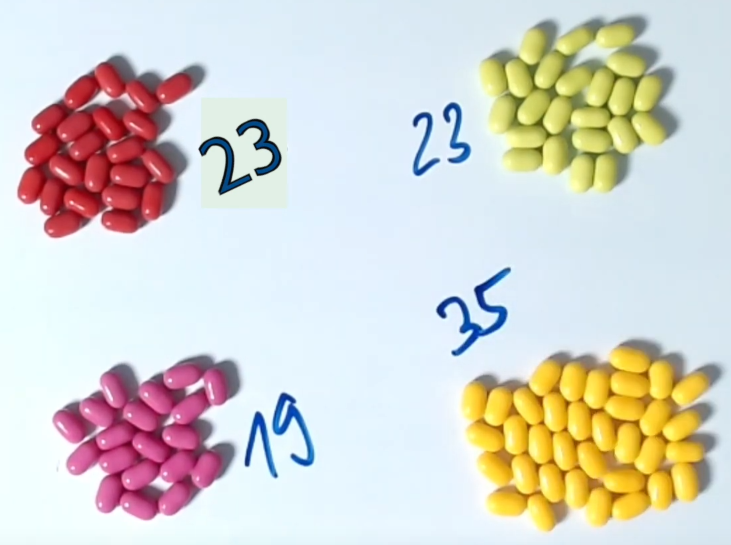
\includegraphics[width=0.8\columnwidth]{Images/tictac}
\end{center}

Damit lässt sich die Diskrepanz berechnen:\\
\begin{center}
	\begin{tabular}{l|rrrrr|}
	Farben $i$ & $p_i$ & $n_i$ & $np_i$ & $n_i - np_i$ & $\frac{(n_i - np_i)^2}{np_i}$ \\ \toprule
	rot & $0.25$ & $23$ & $25$ & $-2$ & $\frac{4}{25}$ \\  \midrule
	pink & $0.25$ & $19$ & $25$ & $-6$ & $\frac{36}{25}$ \\ \midrule
	gelb & $0.25$ & $35$ & $25$ & $10$ & $\frac{100}{25}$ \\ \midrule
	grün & $0.25$ & $23$ & $25$ & $-2$ & $\frac{4}{25}$ \\ \midrule
	& & $n=100$ & & & $D =5.76$ \\ \bottomrule
\end{tabular}
\end{center}

\noindent
$n_i$ Anzahlen, \\
$np_i$ Erwartete Anzahl,  \\
$n_i - np_i$: Abweichungen, \\
$(n_i - np_i)^2/np_i$: Diskrepanz

\subsubsection{Kolmogorov-Smirnof Test}\label{Kolmogorov}
Generiert ein Zufallsgenerator im Intervall $[0, 1]$ mit $\alpha=0.01$ eine gleichverteilte Zufallszahl $x_j$? Damit ist in diesem Beispiel $F(x) = x$ (Lineare Verteilung) und $n$ die Anzahl Werte und $j$ der entsprechender sortierte Eintrag ist.
\begin{center}
	\begin{tabular}{l|r|r|r}
		$j$ & $x_j$ & $\frac{i}{n}-F(x_j)$ & $F(x_j) - \frac{i-1}{n}$ \\ \toprule
		1 & 0.00040 & 0.110 & 0.0004  \\  \midrule
		2& 0.00398 & 0.218 & -0.1071 \\  \midrule
		$\vdots$ & $\vdots$& &  \\  \midrule
		i & 0.43987 & 0.560 &-0.4490 \\ \bottomrule
		& & $\max_1(\dots)$ & $\max_2(\dots)$
	\end{tabular}
\end{center}

Damit ist $\max_1 = 0.61222$ und  $\max_1 = 0.00040$ damit lassen sich die $K$ Werte bestimmen:

\[
K_n^+ = \sqrt{n}\cdot \max_1 = 1.83666 \qquad K_n^- = \sqrt{n}\cdot \max_2 = 0.00120
\]

Weil $K_n^+ > K_\text{krit}$ muss die Hypothese verworfen werden, dass die Zufallszahlen gleichverteilt seien.


\subsection{Fehler von Multi-Sensor-System}
\begin{center}
	\begin{tabular}{l|r|r|r}
		& Messbereich & Std.abweichung $\sigma$ & Grundfreq. \\ \toprule
		Sensor 1 & $\pm37g$ & $24mg \rightarrow 0.024$ & $400$Hz  \\  \midrule
		Sensor 2 & $\pm19g$ & $22mg \rightarrow 0.022$ & $1600$Hz \\  \midrule
	\end{tabular}
\end{center}
Wieviel Prozent kann man den Fehler, gemessen mit der Standardabweichung, maximal korrigieren, wenn man beide Messwerte geeignet mittelt?

Die beiden Sensoren $X_1$ und $X_2$ können mit einer Normalverteilung mit gleichem $\mu$ aber verschiedenen Varienzen gemittelt werden. Ziel ist es die $\var(X)$ zu minimieren. 
\begin{align*}
	X &= tX_1 + (1-t)X_2 \\
	\var(X) &= t^2\var(X_1) + (1-t)^2\var(X_2)
\end{align*}
Das Minimum finden durch Nullsetzten der Ableitung
\begin{align*}
	0 = \frac{d}{dt}\var(X) &= 2t\var(X_1) - 2(1-t)\var(X_2) \\
	\rightarrow  \qquad t &= \frac{\sigma_2^2}{\sigma_1^2 + \sigma_2^2} \\
	 1-t &= \frac{\sigma_1^2}{\sigma_1^2 + \sigma_2^2}
\end{align*}
Ein erste Formel einsetzen
\begin{align*}
	\var(X) &= \left(\frac{\sigma_2^2}{\sigma_1^2 + \sigma_2^2}\right)^2\sigma_1^2 + \left(\frac{\sigma_1^2}{\sigma_1^2 + \sigma_2^2}\right)^2\sigma_2^2 \\
	&= \frac{\sigma_1^2\sigma_2^2}{\sigma_1^2+\sigma_2^2}
\end{align*}
und anschliessend $\sigma$ berechnen
\[
\sigma = \sqrt{\var(X)} = \sqrt{\frac{\sigma_1^2\sigma_2^2}{\sigma_1^2+\sigma_2^2}} = \sqrt{\frac{0.022^2\cdot 0.024^2}{0.022^2 + 0.024^2}} = 0.016
\]  
Man kann also den Fehler von $0.022g$ auf $0.016g$ reduzieren, eine Reduktion um $27\%$.

\subsection{Kalman-Filter}
\todo{Prüfung 2018 Aufgabe 8.}
